%!TEX root = ./intern_report.tex

\subsection{How I got the Opportunity}

\paragraph{}
A long time before the industrial training selection, I had heard Paraqum Technologies was one of the best places to learn about the electronics industry in Sri Lanka and Its CEO, Dr. Ajith Pasqual had taught a module in the university that sparked an interest in me about the subject of silicon design. Therefore, when Paraqum Technologies was listed as an open CV company, I did not hesitate to submit a CV, which got selected by the company staff who then interviewed me thoroughly in their office and sometime later, informed me that I had been selected to the Wave Computing Division.

\paragraph{}
At the start of the Internship, I was placed under the supervision of Eng. Achintha Ihalage, an application engineer whose original task was to handle the timing and constraints of the DPU chip. He walked me through the basics of setting up the Wave Computing workspace, company work ethics and other needed technical skills. He also introduced us to the DPU hardware and other proprietary technologies by Wave. 

\paragraph{}
During the second week, Eng. Henrik Esbensen, who is in charge of the Sri Lankan team at Wave HQ visited the office and demonstrated his ideas for projects. One of these was the Python - Wave Flow Graph translator, also known as Py2WFG. I volunteered to take that project and Eng. Henrik allocated me the necessary resources of the company including support teams and software tools to carry on the project.

\paragraph{}
Working on wave software projects requires high end hardware since it involves performing a lot of repetitive calculations. our laptops are not suitable for this task and therefore I was given access to the central computing grid of wave at the datacenter in Campbell, USA. To utilize these resources, I used a secure shell connection which uses the linux command line of the server and displays it on my laptop via a Virtual Private Network (VPN). Sometimes, this text based interface is not sufficient for the tasks at hand and therefore, a VNC connection had to be used. VNC is much similar to remote desktop found in windows.

\begin{figure}[H]
    \centering
    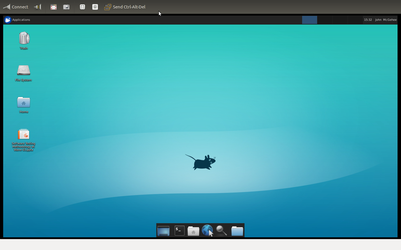
\includegraphics[trim=0cm 0cm 0cm 0cm, clip=true,scale=0.8]{figures/vnc.png}
    \caption{VNC connection view of computing grid\label{Fig:vnc}}\vspace{-4mm}
    \end{figure}

\paragraph{}
This project soon became popular among the crowd of wave computing and I developed it according to the requirements and feedback. The amount of work was rather large but I managed to complete the project and hand it over by the time Internship ended. This project will most likely be adopted by full time developers and expanded to probably replace the existing design flow.

\subsubsection{Notable people at Wave / Paraqum}

\paragraph{}
Wave Computing Sri Lanka is a small workplace with around 15 employees with new people joining often and some leaving for higher studies. It is divided into two main groups, the SDK team I worked with and the application team. The administration structure is explained in detail in Figure \ref{Fig:adminstruct}. 

\begin{figure}[H]
    \centering
    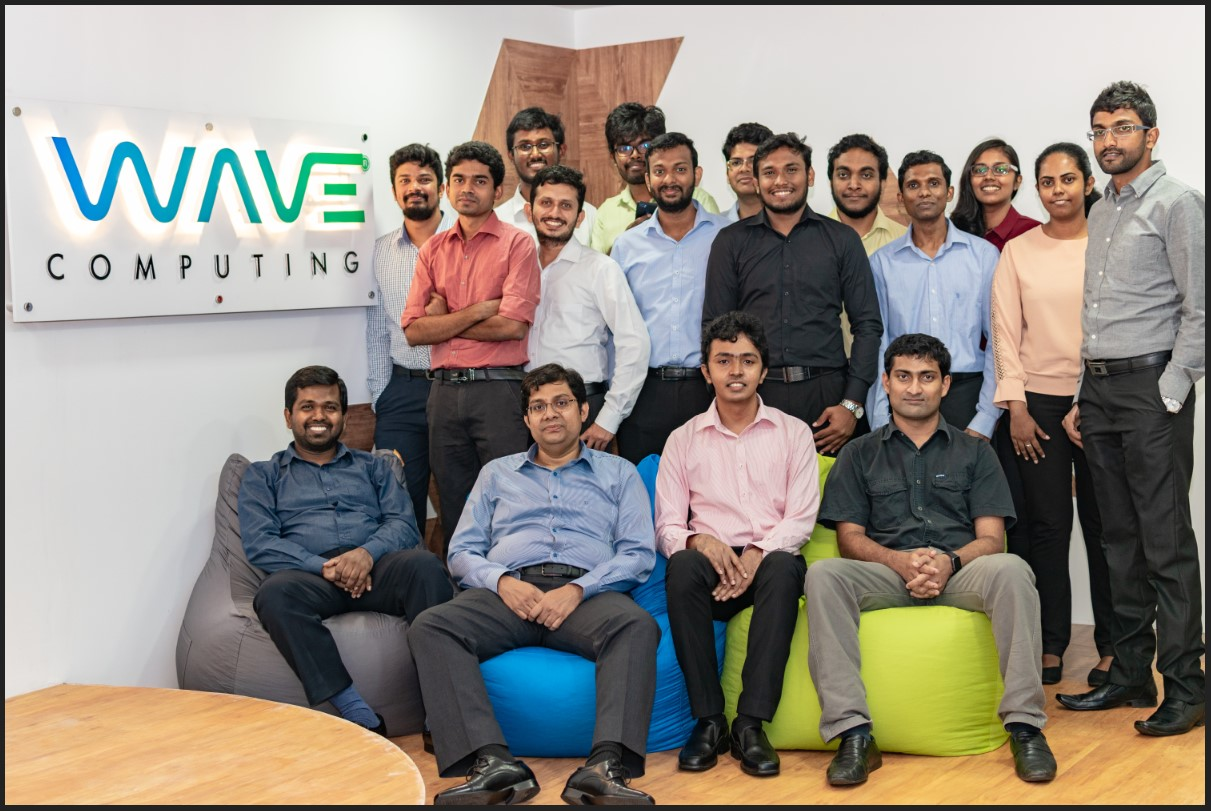
\includegraphics[trim=0cm 0cm 0cm 0cm, clip=true,scale=0.5]{figures/wave_staff.jpg}
    \caption{Wave Computing Sri Lanka staff and Interns at the new office\label{Fig:wavestaff}}\vspace{-4mm}
    \end{figure}

\paragraph{}
Although not a member of the Sri Lankan team, Eng. Henrik Esbensen often visits the Sri Lanka office and is constantly joined with the workflow via online communication channels. He is also the most senior member of Wave computing I have met and worked with. When I took the Py2WFG project, I was placed in his indirect supervision and he has helped me to guide the project to become what it is now and also has given me valuable advice regarding both internship and studies.

\paragraph{}
Wave Sri Lanka is directly managed by Eng. Nuwan Gajaweera, a UoM ENTC graduate engineer with a perfect track record of managing large projects. He is the liaison between Wave HQ and ourselves for any non-technical matter. He is very concerned about the attitude of people towards the workplace and strives to make it a pleasant place for everyone. 

\paragraph{}
The technical leadership of the teams are engineers Upul Ekanayake and Binu Amarathunga, both very highly experienced engineers who have a deep understanding of the project. They are the teams last line of defence against technical issues. One of the reasons for the high efficiency of the Sri Lankan team relative to other teams is this excellent technical leadership.

\paragraph{}
Staff engineer Dakila Serasinghe was my official supervisor for the Py2WFG project. He is one of the first people to create complex designs for the DPU systems. With a deep knowledge on the SDK itself, He helped to resolve numerous problems encountered during the project. Most of the designs I used to test my library on were originally made by him so I could always count on his guidance for issues in work. A critical factor for the on time delivery and the neat design of the Py2WFG is his taste for perfection. 

\paragraph{}
Junior engineers of the Wave application team, Eng. Achintha Ihalage, Eng. Sasindu Wijerathna, Eng. Anton Rathnarajah were our initial supervisors. They were new to the platform so they had recent experience with all the problems we encountered when dealing with the system for the first time. They were the people who always helped us first in any kind of problem. When I received the Py2WFG project and shifted my focus on the SDK team, junior engineers Omega Gamage and Pradeep Kathiragamaraja were the people who helped me out in the field. During the whole period of the internship, they helped us achieve a perfect training experience in any way possible.